\documentclass[11pt]{article}
% Basic Packages for Encoding (Input AND Output) and Langauge Support
\usepackage[utf8]{inputenc}
\usepackage[T1]{fontenc}
\usepackage[french]{babel}

% Change Layout with a User-Friendly Interface
\usepackage[margin=1in]{geometry}

% Include Pictures with a User-Friendly Interface
\usepackage{graphicx}
\usepackage{float}

% Extended Math Support from the Famous 'American Mathematical Society'
\usepackage{amsmath}
\usepackage{amsfonts}
\usepackage{amssymb}

% Just for Demonstration Purposes
\usepackage[math]{blindtext}

% For use on computer
\usepackage{hyperref}

% For table color
\usepackage{xcolor,colortbl}

% Tableau verticale
\usepackage{rotating}

% Titre
\usepackage[affil-it]{authblk}
\title{\textbf{TP Tube de Braun}}
\author{Camille Yerly, Romain Blondel}
\affil{2M8, Gymnase Auguste Piccard}
\date{19 décembre 2022}

\begin{document}

\maketitle

\section{But}

Le but de ce TP est d'étudier la déviation (sur l'écran) d'un faisceau d'électrons en fonction de la tension de déviation $U'$, pour une tension $U$ fixée (aux bornes du canon).

\section{Introduction théorique}

Dans cette expérience, nous utilisons un tube de Braun, soit un canon à électrons. Afin de comprendre le fonctionnement de ce canon, nous allons présenter quelques notions théoriques ci-dessous. Le canon à électron était utilisé, par exemple, dans les anciennes télévisions afin de projeter une image sur l'écran, de nos jours, les écrans LCD ou LED fonctionnent sur d'autres principes. Un montage similaire au tube de Braun est encore utilisé dans les tubes à rayons X, utilisés dans l'imagerie médicale et divers instruments analytiques. Notons que dans ces utilisations l'écran est remplacé par une cible (anode métallique) qui émet du rayonnement dans le domaine des X lorsque qu'elle est frappée par les électrons.
\subsection{Champ électrique}
Le champ électrique est un champ vectoriel distribué autour d'une charge. Dans le tube de Braun, le champ est produit par deux plaques chargées, séparée par une distance. Les charges sont dues à la tension électrique appliquée aux plaques qui cause une accumulation de charges sur une des plaques et un déficit sur l'autre. Cette accumulation/déficit provoque un champ électrique entre les deux plaques. Les plaques étant plates et relativement grandes, elles produisent dans l'espace entre elles un champ quasi-uniforme. Le champ est exprimé en $[V\cdot m^{-1}]$. Selon la position des plaques, les effets du champs diffèrent. Il est ainsi possible soit d'accélérer les électrons lorsque le champ est parallèle à la direction de déplacement des électrons ($U$) ou de changer leur direction lorsque le champ est perpendiculaire ($U'$).
\subsection{Électrons et tension}
Le canon à électrons génère des électrons par le bief d'un filament métallique chauffé. Ils sont ensuite soumis au champ électrique des plaques pour être accélérés et envoyés dans une direction choisie. Augmenter la tension $U$ cause une accélération des électrons, le point lumineux sur l'écran sera donc plus étendu et la déviation possible plus petite. Au contraire, une tension $U$ plus faible produit un point lumineux plus petit et, les électrons allant moins vite, une déviation possible plus large. Changer la tension $U'$, par contre, permet de diriger les électrons. Il est aussi utile de noter que la tension multipliée par la charge, permet d'obtenir l'énergie potentielle d'un système électrique, ce qui permet de relier ça à l'énergie cinétique par exemple, via la loi de conservation de l'énergie ou celle du travail.

\section{Principe de mesure et description}

Le principe est de fixer une feuille de papier millimétré sur l'écran afin de pouvoir mesurer la position du faisceau. Puis de faire mesurer divers couples de valeurs $U$, $U'$ afin d'obtenir diverses vitesses des électrons - sur les variations de $U$ - et donc de changer le temps de passage des électrons entre les plaques de déviation latérale. Ces dernières étant également soumises à diverses tensions $U'$.

\subsection{Matériel}

Afin de réaliser l'expérience, nous avons utilisé :
\begin{itemize}
\item Un tube de Braun monté
\item Deux générateurs de tension
\item Deux voltmètres
\item Une feuille de papier millimétré
\item Divers câbles
\end{itemize}

\subsection{Déroulement}

Le tube de Braun utilisé était déjà monté et câblé. Nous y avons juste ajouté du papier millimétré afin de mesurer la distance/position. Nous avons varié la tension de déviation $U'$ pour trois tensions $U$ aux bornes du canon. 
\begin{enumerate}
\item Nous avons fixée la tension $U$ au maximum que permettait le générateur (612.5 $[V]$).
\item Nous avons effectué des réglages afin de centrer le point de départ des mesures et de focaliser le point lumineux (cela n'est néanmoins pas parfait à cause du papier et il faut estimer à peu près le centre de la tache). 
\item A l'aide d'un papier millimétré, nous avons varié la tension $U'$ afin de relever plusieurs mesures de la déviation à des intervalles de distances réguliers.
\item Nous avons réitéré l'étape 3 pour deux autres $U$ (450 et 380.4 $[V]$, la tension minimale du générateur).
\end{enumerate}

\subsection{Schéma}

\begin{figure}[H]
\center
 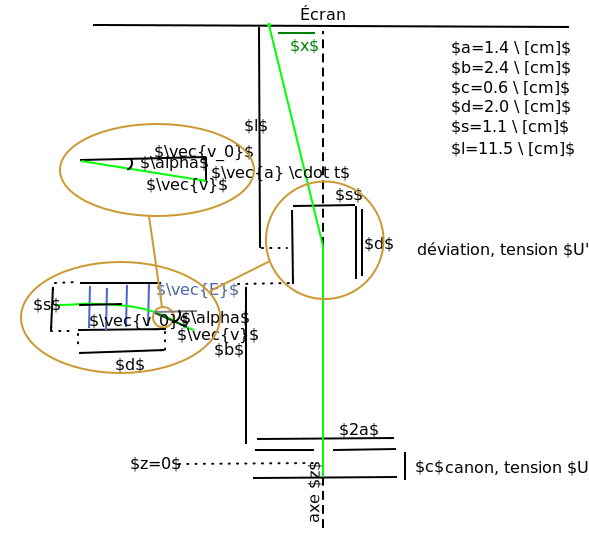
\includegraphics[scale=1]{Images/schm-th.pdf}
\caption{Schéma théorique de l'expérience}
\label{fig:schm-th}
\end{figure}

\section{Résultats et calculs}

Nous avons donc mesurer la position sur l'écran selon la tension du canon et celle de déviation. Nous considérons comme référentiel une position du même signe que la tension de déviation, et la tension du canon est toujours positive.\\ \\
Doté de ces mesures, il est intéressant de de la comparer avec les résultats théorique. Pour toute la nomenclature, nous nous référerons à la figure \ref{fig:schm-th}.\\
Tout d'abord, il faut prendre en compte que l'électron freine en quittant le canon, et qu'il faut donc prendre sa tension d’accélération $U_{acc}$, plus petit que $U$, dans les calculs. Afin de la calculer, nous nous basons sur le potentiel normalisé $V(z)=f(z - \frac{c}{2})-f(z+\frac{c}{2})$  avec $f(z)=\sqrt{1+(\frac{z}{a})^2}-\frac{|z|}{a}$ (voir figure \ref{fig:u-norm}). Alors, la tension normalisée de $U$ correspond à la différence de potentiel entre la plaque du canon (en $-\frac{c}{2}$) et le trou (en $\frac{c}{2}$), soit $V(\frac{c}{2})-V(-\frac{c}{2})$. Celle de $U_{acc}$ correspond par la même réflexion à celle entre le début du canon et l'entrée entre les plaques de déviation (en $b+\frac{c}{2}$), donc $V(b+\frac{c}{2})-V(-\frac{c}{2})$. De là, on peut connaître le rapport $\frac{U}{U_{acc}}=\frac{V(\frac{c}{2})-V(-\frac{c}{2})}{V(b+\frac{c}{2})-V(-\frac{c}{2})} \approx 1.751$. Il est ensuite relativement aisé de trouver $U_{acc} = \frac{U}{(\frac{U}{U_{acc}})}$.

\begin{figure}[H]
\center
\includegraphics[scale=0.75]{Images/tens-norm.pdf}
\caption{Graphe de la tension normalisée $V(z)$}
\label{fig:u-norm}
\end{figure}

Maintenant que ce préambule est fixé, passons au calcul à proprement parlé. Par la conservation de l'énergie, celle donnée par la tension d'accélération est égal à celle cinétique à l'entrée des plaques de déviations (on considéreras ensuite sa vitesse $v_0$ selon $z$ constante) : $-e \cdot (-U_{acc}) = \frac{1}{2} \cdot m \cdot v_0^2 \Leftrightarrow v_0 = \sqrt{\frac{2 \cdot e \cdot U_{acc}}{m}}$ avec $e$ la charge de l'électron et $m$ sa masse. Dans le champ de déviation $E = \frac{U'}{s}$, l'électron subit une force $F=m \cdot a$ selon Newton, mais $F=e \cdot E$ par définition du champ électrique. En regroupant les deux on peut calculer l'accélération de la particule entre les deux plaques $m \cdot a = e \cdot E \Leftrightarrow a = \frac{e \cdot E}{m} = \frac{e \cdot U'}{m \cdot s}$. Comme on considère la vitesse constante, le temps de passage entre les deux plaques sera $t = \frac{d}{v_0}$. La composante verticale de la vitesse $v$ à la sortie est donc $a \cdot t$, et nous pouvons donc établir la relation de entre l'angle de déviation et le reste $\tan \alpha = \frac{a \cdot t}{v_0} = \frac{a \cdot d}{v_0^2} = \frac{\frac{e \cdot U'}{m \cdot s}\cdot d}{\frac{2 \cdot e \cdot U_{acc}}{m}} = \frac{d}{2s}\frac{U'}{U_{acc}}$. Par la géométrie du système, on peut poser également que $\tan \alpha \approx \frac{x}{l}$. Finalement, on obtient $\frac{x}{l} = \frac{d}{2s}\frac{U'}{U_{acc}} \Leftrightarrow x = \frac{ld}{2s}\frac{U'}{U_{acc}}$. Vu que lors de l'expérience on avait une distance fixée, nous avons calculé la tension que nous devrions obtenir via $U' = \frac{2sx}{ld}\cdot U_{acc}$.\\ \\
Dans les tables ci-dessous (tables \ref{table:u_612}, \ref{table:u_450} et \ref{table:u_308}) sont consignés la tension mesurée $U'$ pour obtenir la distance $x$, ainsi que celle théorique, pour différentes tensions $U$. Il y est également mentionné l'erreur relative entre la tension théorique et celle mesurée : $|\frac{U'_{mes}-U'_{th}}{U'_{th}}|$.

\begin{table}[H]
\center
\begin{tabular}{|c|>{\columncolor{lightgray}}c|c|>{\columncolor{lightgray}}c|}
\hline
\rowcolor{gray} Distance $[cm]$ & Tension mesurée $[V]$ & Tension théorique $[V]$ & Erreur $[\%]$ \\ \hline
-2.4 & -79.3 & -80.32 & 1.26 \\ \hline
-2 & -65.9 & -66.93 & 1.54 \\ \hline
-1.5 & -50.08 & -50.2 & 0.23 \\ \hline
-1 & -34.63 & -33.46 & 3.48 \\ \hline
-0.5 & -18.12 & -16.73 & 8.29 \\ \hline
0 & 0 & 0.0 & 0 \\ \hline
0.5 & 19.6 & 16.73 & 17.14 \\ \hline
1 & 35.9 & 33.46 & 7.28 \\ \hline
1.5 & 52.3 & 50.2 & 4.19 \\ \hline
2 & 69 & 66.93 & 3.09 \\ \hline
2.2 & 75.2 & 73.62 & 2.14 \\ \hline
\end{tabular}
\caption{Mesure de distance, tension ainsi que calcul de la tension théorique et de l'erreur pour $U=612.5 \ [V]$ ($U_{acc} = 349.858 [V]$)}
\label{table:u_612}
\end{table}

\begin{table}[H]
\center
\begin{tabular}{|c|>{\columncolor{lightgray}}c|c|>{\columncolor{lightgray}}c|}
\hline
\rowcolor{gray} Distance $[cm]$ & Tension mesurée $[V]$ & Tension théorique $[V]$ & Erreur $[\%]$ \\ \hline
-3.3 & -78 & -81.13 & 3.86 \\ \hline
-3 & -70 & -73.76 & 5.1 \\ \hline
-2.5 & -58.7 & -61.47 & 4.5 \\ \hline
-2 & -48 & -49.17 & 2.38 \\ \hline
-1.5 & -37.15 & -36.88 & 0.73 \\ \hline
-1 & -25.15 & -24.59 & 2.29 \\ \hline
-0.5 & -12.16 & -12.29 & 1.08 \\ \hline
0 & 0 & 0.0 & 0 \\ \hline
0.5 & 14.9 & 12.29 & 21.21 \\ \hline
1 & 27.15 & 24.59 & 10.43 \\ \hline
1.5 & 38.55 & 36.88 & 4.53 \\ \hline
2 & 50.78 & 49.17 & 3.27 \\ \hline
2.5 & 63.6 & 61.47 & 3.47 \\ \hline
3 & 75.2 & 73.76 & 1.95 \\ \hline
\end{tabular}
\caption{Mesure de distance, tension ainsi que calcul de la tension théorique et de l'erreur pour $U=450 \ [V]$ ($U_{acc} = 257.039 [V]$)}
\label{table:u_450}
\end{table}

\begin{table}[H]
\center
\begin{tabular}{|c|>{\columncolor{lightgray}}c|c|>{\columncolor{lightgray}}c|}
\hline
\rowcolor{gray} Distance $[cm]$ & Tension mesurée $[V]$ & Tension théorique $[V]$ & Erreur $[\%]$ \\ \hline
-4 &   -61.9 & -67.4 & 8.16 \\ \hline
-3.5 & -53.63 & -58.97 & 9.06 \\ \hline 
-3 &  -47.67 & -50.55 & 5.7 \\ \hline
-2.5 & -41.55 & -42.12 & 1.36 \\ \hline 
-2 &  -32.84 & -33.7 & 2.55 \\ \hline
-1.5 & -25.18 & -25.27 & 0.37 \\ \hline 
-1 &  -17.2 & -16.85 & 2.08 \\ \hline
-0.5 & -8.28 & -8.42 & 1.72 \\ \hline 
0 &  0 & 0.0 & 0 \\ \hline
0.5 &  10.4 & 8.42 & 23.44 \\ \hline
1 &  19.12 & 16.85 & 13.47 \\ \hline
1.5 &  27.65 & 25.27 & 9.4 \\ \hline
2 &  35.79 & 33.7 & 6.2 \\ \hline
2.5 &  42.6 & 42.12 & 1.13 \\ \hline
3 &  50.62 & 50.55 & 0.14 \\ \hline
3.5 &  59.32 & 58.97 & 0.59 \\ \hline
4 &  66.9 & 67.4 & 0.74 \\ \hline
\end{tabular}
\caption{Mesure de distance, tension ainsi que calcul de la tension théorique et de l'erreur pour $U=308.4 \ [V]$ ($U_{acc} = 176.157 [V]$)}
\label{table:u_308}
\end{table}

Dans la figure \ref{fig:dist-u}, nous avons tracé la distance selon la tension de déviation pour nos différentes tensions dans le canon, ainsi que mis les points correspondant à nos mesures.

\begin{figure}[H]
\center
\includegraphics[scale=0.75]{Images/sim-real.pdf}
\caption{Graphe de la distance $x$ selon la tension $U'$}
\label{fig:dist-u}
\end{figure}

Afin de pouvoir mieux comparer nos résultats d'erreur, la figure \ref{fig:hist-err} est un histogramme de celle-ci, ainsi que les moyennes (dans l'ordre décroissant des tensions : $4.42 \ [\%]$, $4.63 \ [\%]$ et $5.07 \ [\%]$, ce qui donne sur toute les mesures $4.75 \ [\%]$) pour les groupes de mesures et celle globale.

\begin{figure}[H]
\center
\includegraphics[scale=0.75]{Images/erreur-hist.pdf}
\caption{Histogramme des erreurs}
\label{fig:hist-err}
\end{figure}

\section{Discussion des résultats}

Les résultats sont globalement assez proches du modèle théorique. Comme nous le voyons sur la figure \ref{fig:dist-u}, la distance sur l'écran et linéairement proportionnelle à la tension de déviation. On remarque que pour la tension $U = 308.4 \ [V]$, les distances de signe négative sont celles avec le plus d'écart avec les droites. Cela peut s'expliquer par le fait que le tube de Braun que l'on a utilisé n'est pas parfait. Lorsque l'on a placé le papier millimétré, on à constaté que la déviation n'est pas parfaitement rectiligne, mais qu'elle fait un peu une courbe. Cela explique peut être le fait que ça impacte plus cette mesure qui se déroulait sur une plus grande plage de position.\\ \\
Néanmoins, on constate que en erreur relative ce ne sont pas non plus des différences complètement étonnantes. En effet, elles sont de faibles précision ($\sim 10 \ [\%]$), mais il y a des mesures qui sont bien plus imprécise selon la figure \ref{fig:hist-err}. Il faut quand même noter que toutes les mesures associées à des erreurs supérieurs à $10 \ [\%]$ sont pour des distances proches de zéro ($0.5$ et $1.0 \ [cm]$), et donc d'une part avec des tensions faibles mais d'autre part, et surtout, avec de petites distances. Si l'on regarde sur les tables \ref{table:u_612}, \ref{table:u_450} et \ref{table:u_308}, on constate que ces mesures ont une erreur absolue de l'ordre de $2$ ou $3 \ [V]$, ce qui correspond à celle des autres mesures, donc c'est principalement le faible ordre de grandeur qui crée des aussi grandes erreurs relatives.\\
Pourtant, sur la moyenne, les mesures sont d'une précision acceptable ($\sim 5 \ [\%]$), et il y a une majorité de mesures qui sont de bonne précision et d'excellente précision ($\sim 2 \ [\%]$), malgré l'imprécision liée à la diffraction du point lumineux dans le papier millimétré.\\ \\
Finalement, il y a des approximations dans le modèle théorique qui peuvent expliquer certaines choses. Tout d'abord, l'importance d'avoir utilisé une tension d'accélération plutôt que directement celle du canon (celle-ci est $\sim 40 \ [\%]$ moindre que celle du canon). Mais c'est une formule donnée tel quel qui pourrait être affinée pour chaque dispositif, comme les dimensions qui sont celle donnée par le protocole (ou le fabricant), mais on ne sait pas à quel point elles sont exactes. \\
Ensuite, la formule utilisée ($x = \frac{ld}{2s}\frac{U'}{U_{acc}}$) à des avantages, mais elle fait quelques approximation. En effet, nous considérons que c'est un triangle rectangle de cathètes $x$ et $l$. Ceci est une excellente approximations, au vu des résultats, mais si l'on souhaitait être exacte, il aurait fallu prendre $x - \frac{1}{2} a \cdot t^2$ (selon le mouvement rectiligne uniformément accéléré) et $l - \frac{d}{2}$. Mais ceci n'est pas vraiment préférable, car les simplifications de la masse et la charge de l'électron ne serait pas faisable, et donc l'expérience perd un peu de son intérêt vu que l'on devrait se baser sur d'autres mesures ou des tables. De plus, l'approximation faite est excellente en plus d'être pratique, car le faible temps de passage de l'électron et la grande accélération font que cela est très proche de la réalité.

\section{Conclusion}

En conclusion, les résultats obtenus sont très satisfaisant. La précision y est très acceptable, et le modèle mathématique offre des approximations pratiques et presque esthétique. L'expérience peut être modifiée afin de dévier l'électron sur deux dimensions en ajoutant une seconde paire de plaques de déviation. On peut aussi essayer un tube qui utilise des aimants afin de dévier le faisceau d'électron, en ayant remarqué par curiosité qu'un aimant le faisait bouger de manière plus efficace. De plus, une grille imprimée directement sur le tube, ou une gille sans papier millimétré, permettrais d'éviter la diffraction du rayon et offrirait donc une meilleure précision. Il pourrait aussi être intéressant d'utiliser ce dispositif afin de visualiser d'autres chose, comme par exemple les variation de tension d'un système.

\end{document}